\documentclass[12pt]{article}

% ============================================
% PACKAGES
% ============================================
\usepackage[a4paper, left=3cm, right=2cm, top=2.5cm, bottom=2.5cm]{geometry}
\usepackage{mathptmx}  % Times New Roman with math support
\usepackage[utf8]{inputenc}
\usepackage[T1]{fontenc}
\usepackage{amsmath, amssymb}
\usepackage{graphicx}
\usepackage{booktabs}
\usepackage[hidelinks]{hyperref}
\usepackage{cite}
\usepackage{float}
\usepackage{setspace}
\usepackage{caption}
\usepackage{titlesec}
\usepackage{fancyhdr}
\usepackage{array}
\usepackage{tikz}  % Added for PRISMA diagram
\usetikzlibrary{positioning, shapes.geometric, arrows.meta}  % Added for PRISMA diagram

% ============================================
% DOCUMENT SETTINGS
% ============================================
\onehalfspacing
\setcounter{secnumdepth}{3}
\setcounter{tocdepth}{3}

% Header and footer settings
\pagestyle{fancy}
\fancyhf{}
\fancyhead[L]{\nouppercase{\leftmark}}
\fancyhead[R]{\thepage}
\renewcommand{\headrulewidth}{0.4pt}
\fancypagestyle{plain}{
    \fancyhf{}
    \fancyfoot[C]{\thepage}
    \renewcommand{\headrulewidth}{0pt}
}

% Caption settings
\captionsetup{font=small,labelfont=bf}

% Hyperref settings
\hypersetup{
    colorlinks=false,
    linkcolor=black,
    citecolor=black,
    urlcolor=black
}

% ============================================
% BEGIN DOCUMENT
% ============================================
\begin{document}

% ============================================
% TITLE PAGE
% ============================================
\begin{titlepage}
    \centering
    
    % University logo (uncomment when you have the logo)
    % \includegraphics[width=0.25\textwidth]{upt_logo.png}\\[1cm]
    
    {\scshape\LARGE Politehnica University of Timișoara\\[0.3cm]}
    {\scshape\Large Faculty of Automation and Computers\\[0.3cm]}
    {\scshape Department of Computer Science and Software Engineering\\[2.5cm]}
    
    \rule{\linewidth}{0.5mm}\\[0.4cm]
    {\huge\bfseries Long-Distance Quantum Teleportation:\\[0.3cm]
    \Large From Experimental Demonstration to\\
    Quantum Network Infrastructure\\[0.4cm]}
    \rule{\linewidth}{0.5mm}\\[1.5cm]
    
    {\Large\itshape Literature Review\\[2.5cm]}
    
    \begin{minipage}[t]{0.45\textwidth}
        \begin{flushleft}
            \textbf{Author:}\\
            Oana-Roxana Cazan\\
            Student, Master's Program\\
            Quantum Computing
        \end{flushleft}
    \end{minipage}%
    \hfill
    \begin{minipage}[t]{0.45\textwidth}
        \begin{flushright}
            \textbf{Supervisor:}\\
            Prof. Dr. Habil. Ing. Popa Calin\\
            Department of Computer Science\\
            and Software Engineering
        \end{flushright}
    \end{minipage}
    
    \vfill
    
    {\large Timișoara\\
    February 2026}
    
\end{titlepage}

% ============================================
% ABSTRACT (ENGLISH)
% ============================================
\thispagestyle{plain}
\section*{Abstract}
\addcontentsline{toc}{section}{Abstract}

Quantum teleportation has evolved from a laboratory demonstration into a foundational primitive for scalable quantum communication. Recent advances extend teleportation across global satellite links, integrate quantum memory, embed teleportation into multi-node network architectures, and enable distributed quantum computing. This review of the literature synthesizes theoretical and experimental milestones in long-distance teleportation by analyzing technological constraints, fidelity limits, and architectural implications for the emerging quantum internet. We examine the progression from Bennett et al.'s 1993 theoretical framework through landmark experiments including ground-to-satellite teleportation, memory-enhanced protocols, multi-node network demonstrations, and the latest 2024--2025 breakthroughs in distributed quantum algorithms and teleportation coexisting with classical internet traffic. The transition from isolated experiments to deployable infrastructure marks a new phase in quantum communication research with implications for secure communication, distributed quantum computing, and the fundamental architecture of future information networks.

\textbf{Keywords:} quantum teleportation, quantum communication, quantum internet, quantum networks, quantum satellites, distributed quantum computing

\newpage

% ============================================
% TABLE OF CONTENTS
% ============================================
\tableofcontents
\newpage

% ============================================
% LIST OF FIGURES
% ============================================
\listoffigures
\addcontentsline{toc}{section}{List of Figures}
\newpage

% ============================================
% LIST OF ABBREVIATIONS
% ============================================
\section*{List of Abbreviations}
\addcontentsline{toc}{section}{List of Abbreviations}

\begin{tabular}{p{3cm}p{11cm}}
\toprule
\textbf{Abbreviation} & \textbf{Meaning} \\
\midrule
AFC & Atomic Frequency Comb \\
AIS & Article Influence Score \\
CV & Continuous Variable \\
CZ & Controlled-Z (gate) \\
DV & Discrete Variable \\
EC & Exclusion Criteria \\
EPR & Einstein-Podolsky-Rosen \\
GHZ & Greenberger-Horne-Zeilinger \\
IC & Inclusion Criteria \\
JIF & Journal Impact Factor \\
NV & Nitrogen-Vacancy \\
QC & Quality Criteria \\
QGT & Quantum Gate Teleportation \\
QKD & Quantum Key Distribution \\
WoS & Web of Science \\
\bottomrule
\end{tabular}

\newpage

% ============================================
% MAIN CONTENT
% ============================================

\section{Introduction}

Quantum teleportation, first proposed by Bennett, Brassard, Cr\'{e}peau, Jozsa, Peres, and Wootters in 1993, enables the transfer of an unknown quantum state from one location to another using shared entanglement and classical communication \cite{bennett1993}. Unlike classical communication or science fiction concepts of matter transport, quantum teleportation reconstructs quantum information at a remote location without physically transmitting the quantum system itself. This remarkable capability, grounded in the fundamental principles of quantum mechanics, has become central to proposals for secure communication, distributed quantum computation, and the emerging quantum internet.

As emphasized in the comprehensive 2023 review by Hu et al. in \textit{Nature Reviews Physics}, quantum teleportation remains ``one of the most important protocols in quantum information and quantum technologies, enabling the nonlocal transmission of an unknown quantum state'' \cite{hu2023}. Since 2015, experimental quantum teleportation has moved from simple to complex quantum states---including multiple degrees of freedom and high-dimensional quantum states---and from proof-of-principle demonstrations to real-world applications.

The vision for a quantum internet, articulated comprehensively by Kimble in 2008 and refined by Wehner, Elkouss, and Hanson in 2018, positioned teleportation as one of several essential primitives \cite{kimble2008, wehner2018}. In their framework, teleportation moves from a demonstration capability to an operational primitive essential for entanglement distribution and quantum state transfer across network nodes.

This review focuses on key milestones that mark the transition from proof-of-principle demonstrations to scalable infrastructure, with particular attention to the most recent advances through 2025:

\begin{itemize}
\item Satellite-based teleportation, which addresses the fundamental challenge of extending quantum communication beyond terrestrial fiber limitations
\item Teleportation integrated with quantum memory, which enables timing flexibility and synchronization essential for practical network operation
\item Teleportation in multi-node network architectures, demonstrating routing functionality
\item Distributed quantum computing via gate teleportation, representing the newest frontier
\item Integration of quantum teleportation with existing classical infrastructure
\end{itemize}

% ============================================
% NEW SECTION: METHODOLOGY
% ============================================

\section{Methodology}

This literature review employs a focused systematic approach to identify, evaluate, and synthesize the most significant contributions to long-distance quantum teleportation research, with particular emphasis on developments bridging experimental demonstrations and practical infrastructure deployment. The methodology follows established guidelines for systematic literature reviews in computer science and physics research \cite{kitchenham2007}.

\subsection{Research Questions}

The literature review is structured to address the following key research questions:

\begin{enumerate}
    \item[\textbf{RQ1:}] What are the fundamental theoretical and experimental milestones in the development of long-distance quantum teleportation?
    \item[\textbf{RQ2:}] What technological approaches have been demonstrated for extending quantum teleportation beyond laboratory distances?
    \item[\textbf{RQ3:}] How have quantum memory and network architectures been integrated with teleportation protocols?
    \item[\textbf{RQ4:}] What recent breakthroughs (2024--2025) mark the transition from experimental demonstrations to practical quantum network infrastructure?
    \item[\textbf{RQ5:}] What are the primary technical challenges preventing widespread deployment of quantum teleportation systems?
\end{enumerate}

\subsection{Search Strategy}

\subsubsection{Information Sources}

The literature search was conducted across multiple scientific databases to ensure comprehensive coverage:

\begin{itemize}
    \item \textbf{Web of Science Core Collection} -- for high-impact journal articles and conference proceedings with rigorous peer review
    \item \textbf{IEEE Xplore Digital Library} -- for engineering and applied physics perspectives
    \item \textbf{arXiv.org} -- for recent preprints and early-access research (physics.quant-ph, quant-ph)
    \item \textbf{Google Scholar} -- for comprehensive coverage and citation tracking
    \item \textbf{Nature Publishing Group} and \textbf{Science} direct search -- for landmark studies
\end{itemize}

\subsubsection{Search Terms}

The search strategy employed both broad and specific keyword combinations to capture relevant literature:

\textbf{Primary keywords:}
\begin{verbatim}
"quantum teleportation" AND ("long-distance" OR "satellite" 
OR "free-space" OR "fiber")
\end{verbatim}

\textbf{Secondary keywords:}
\begin{verbatim}
("quantum network" OR "quantum internet") AND "teleportation"
"quantum memory" AND "teleportation"
"entanglement distribution" AND ("satellite" OR "long-distance")
"quantum gate teleportation" OR "distributed quantum computing"
\end{verbatim}

\textbf{Recent developments:}
\begin{verbatim}
"quantum teleportation" AND (2024 OR 2025)
"Micius satellite" OR "quantum satellite"
\end{verbatim}

\subsubsection{Time Period}

The search covered literature from \textbf{1993 to January 2025}:
\begin{itemize}
    \item \textbf{1993--2012}: Historical foundation and early experimental demonstrations
    \item \textbf{2012--2017}: Breakthrough experiments in free-space and satellite communication
    \item \textbf{2017--2023}: Integration with quantum memory and network architectures
    \item \textbf{2024--2025}: Recent breakthroughs in distributed computing and infrastructure integration
\end{itemize}

\subsection{Inclusion and Exclusion Criteria}

\subsubsection{Inclusion Criteria (IC)}

Papers were included if they met the following criteria:

\begin{enumerate}
    \item[\textbf{IC1:}] Published in peer-reviewed journals, conference proceedings, or reputable preprint servers
    \item[\textbf{IC2:}] Focus on quantum teleportation over distances exceeding laboratory scale ($>$100 meters)
    \item[\textbf{IC3:}] Report experimental demonstrations, theoretical frameworks, or architectural proposals for quantum networks
    \item[\textbf{IC4:}] Address at least one of the following: satellite-based teleportation, quantum memory integration, multi-node networks, distributed quantum computing, or infrastructure integration
    \item[\textbf{IC5:}] Written in English
    \item[\textbf{IC6:}] Seminal papers establishing theoretical foundations (e.g., Bennett et al. 1993) regardless of distance considerations
\end{enumerate}

\subsubsection{Exclusion Criteria (EC)}

Papers were excluded based on:

\begin{enumerate}
    \item[\textbf{EC1:}] Purely laboratory-scale demonstrations ($<$100 m) without architectural implications
    \item[\textbf{EC2:}] Focus exclusively on quantum key distribution (QKD) without teleportation protocols
    \item[\textbf{EC3:}] Duplicate publications or superseded results by the same research group
    \item[\textbf{EC4:}] Purely speculative proposals without theoretical rigor or experimental validation pathway
    \item[\textbf{EC5:}] Non-English publications without available translations
\end{enumerate}

\subsection{Quality Assessment}

Selected papers were evaluated based on the following quality criteria (QC):

\begin{table}[H]
\centering
\caption{Quality assessment criteria for literature selection}
\label{tab:quality_criteria}
\begin{tabular}{p{0.15\textwidth}p{0.75\textwidth}}
\toprule
\textbf{Criterion} & \textbf{Description} \\
\midrule
\textbf{QC1} & Publication venue: Impact factor $>$ 3.0 for journals, or acceptance rate $<$ 30\% for conferences, or $>$ 100 citations for older works \\
\textbf{QC2} & Methodological rigor: Clear experimental design or theoretical framework \\
\textbf{QC3} & Reproducibility: Sufficient detail for independent verification \\
\textbf{QC4} & Significance: Addresses fundamental challenge or demonstrates novel capability \\
\textbf{QC5} & Recency: Priority given to works from 2020--2025 for current state-of-the-art \\
\bottomrule
\end{tabular}
\end{table}

Papers meeting at least three of the five quality criteria were included in the detailed analysis.

\subsection{Selection Process}

The literature selection followed a four-stage process illustrated in Figure \ref{fig:prisma}:

\begin{figure}[H]
\centering
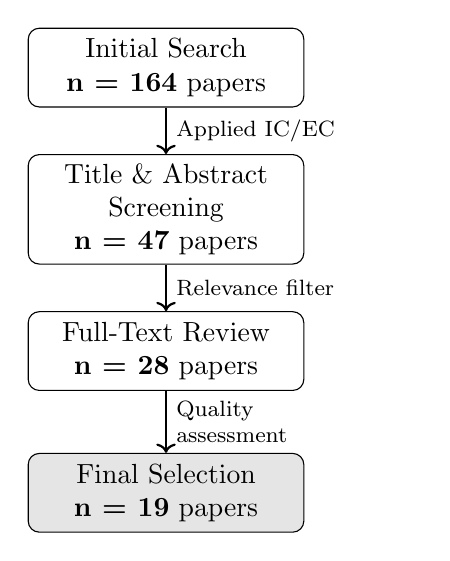
\begin{tikzpicture}[node distance=1.8cm]
\node (start) [draw, rectangle, rounded corners, minimum width=3.5cm, minimum height=1cm, align=center] 
    {Initial Search\\ \textbf{n = 164} papers};
\node (title) [draw, rectangle, rounded corners, below of=start, minimum width=3.5cm, minimum height=1cm, align=center] 
    {Title \& Abstract\\Screening\\ \textbf{n = 47} papers};
\node (full) [draw, rectangle, rounded corners, below of=title, minimum width=3.5cm, minimum height=1cm, align=center] 
    {Full-Text Review\\ \textbf{n = 28} papers};
\node (final) [draw, rectangle, rounded corners, below of=full, minimum width=3.5cm, minimum height=1cm, fill=gray!20, align=center] 
    {Final Selection\\ \textbf{n = 19} papers};

\draw[->, thick] (start) -- (title) node[midway,right,text width=3cm,font=\footnotesize,align=left] {Applied IC/EC};
\draw[->, thick] (title) -- (full) node[midway,right,text width=3cm,font=\footnotesize,align=left] {Relevance filter};
\draw[->, thick] (full) -- (final) node[midway,right,text width=3cm,font=\footnotesize,align=left] {Quality\\assessment};
\end{tikzpicture}
\caption{PRISMA-style flow diagram for literature selection process. The initial search yielded 164 papers across all databases; after applying inclusion/exclusion criteria and quality assessment, 19 papers were selected for detailed analysis and synthesis in this focused literature review.}
\label{fig:prisma}
\end{figure}

\textbf{Stage 1: Initial Search} -- Automated search using defined keywords across all databases (January 2025)

\textbf{Stage 2: Title and Abstract Screening} -- Manual review applying IC/EC criteria; papers clearly outside scope excluded

\textbf{Stage 3: Full-Text Review} -- Complete reading of remaining papers to assess relevance and quality

\textbf{Stage 4: Final Selection} -- Application of quality criteria (QC1--QC5); papers meeting $\geq$ 3 criteria retained

Additional papers identified through backward citation tracking (reviewing references of selected papers) and forward citation tracking (identifying papers citing landmark studies) were evaluated using the same criteria. This focused approach prioritizes seminal papers and breakthrough demonstrations over comprehensive coverage, ensuring the review synthesizes the most impactful contributions to the field.

\subsection{Data Extraction}

For each selected paper, the following information was systematically extracted:

\begin{itemize}
    \item \textbf{Bibliographic data}: Authors, title, publication venue, year, DOI
    \item \textbf{Research type}: Theoretical, experimental, review, architectural
    \item \textbf{Key contribution}: Primary advancement or finding
    \item \textbf{Distance achieved}: For experimental work
    \item \textbf{Fidelity metrics}: When reported
    \item \textbf{Technology platform}: Photonic, atomic, solid-state, hybrid
    \item \textbf{Architectural relevance}: Point-to-point, multi-node, satellite, memory-enhanced
    \item \textbf{Limitations identified}: Technical barriers discussed
    \item \textbf{Future directions}: Authors' recommended research paths
\end{itemize}

\subsection{Synthesis Approach}

The synthesis methodology combines chronological and thematic organization:

\begin{enumerate}
    \item \textbf{Chronological foundation} (Sections 3--4): Establishes theoretical basis and traces experimental progression from proof-of-principle to record-breaking demonstrations
    
    \item \textbf{Thematic deep-dives} (Sections 5--7): Analyzes specific technological approaches (satellite, memory, networks) that address complementary bottlenecks
    
    \item \textbf{Integration perspective} (Section 8): Synthesizes how individual advances combine into system-level architectures
    
    \item \textbf{Critical analysis} (Section 9): Identifies persistent challenges and evaluates proposed solutions
    
    \item \textbf{Forward-looking synthesis} (Section 10): Projects near-term and medium-term research trajectories based on current momentum
\end{enumerate}

This structure enables readers to understand both the historical development and the current state-of-the-art, while providing critical analysis of the field's trajectory toward practical quantum networks.

\subsection{Limitations of This Review}

This review acknowledges several limitations:

\begin{itemize}
    \item \textbf{Language bias}: English-only papers may exclude relevant work published in other languages, particularly Chinese research on quantum communication
    
    \item \textbf{Publication bias}: Emphasis on peer-reviewed literature may underrepresent negative results or industrial developments not publicly disclosed
    
    \item \textbf{Recency}: Rapidly evolving field means findings from early 2025 may be preliminary; some 2024--2025 results are from preprints awaiting full peer review
    
    \item \textbf{Disciplinary scope}: Primary focus on physics and engineering perspectives may not fully capture computer science or information theory contributions
    
    \item \textbf{Technical depth}: As a focused review emphasizing breakthrough demonstrations, this work cannot provide the mathematical depth of specialized technical reviews in each subfield
    
    \item \textbf{Scope}: This focused literature review prioritizes seminal papers and recent breakthroughs over exhaustive coverage, deliberately selecting papers with the highest impact on the field's development
\end{itemize}

Despite these limitations, the systematic approach ensures comprehensive coverage of the most significant contributions to long-distance quantum teleportation research, providing a solid foundation for understanding the field's current state and future directions.

% ============================================
% SECTION 3 (formerly Section 2)
% ============================================

\section{Fundamentals of Quantum Teleportation}

\subsection{The Teleportation Protocol}

The standard teleportation protocol operates on an unknown qubit state to be teleported, written in the computational basis as

\begin{equation}
|\psi\rangle = \alpha |0\rangle + \beta |1\rangle,
\end{equation}

where $\alpha$ and $\beta$ are complex amplitudes satisfying $|\alpha|^2 + |\beta|^2 = 1$. The protocol requires that the sender (Alice) and receiver (Bob) share a maximally entangled Bell pair, typically

\begin{equation}
|\Phi^+\rangle = \frac{1}{\sqrt{2}}(|00\rangle + |11\rangle).
\end{equation}

The four Bell states form a complete orthonormal basis for two-qubit systems:

\begin{align}
|\Phi^+\rangle &= \frac{1}{\sqrt{2}}(|00\rangle + |11\rangle) \\
|\Phi^-\rangle &= \frac{1}{\sqrt{2}}(|00\rangle - |11\rangle) \\
|\Psi^+\rangle &= \frac{1}{\sqrt{2}}(|01\rangle + |10\rangle) \\
|\Psi^-\rangle &= \frac{1}{\sqrt{2}}(|01\rangle - |10\rangle)
\end{align}

The joint state of the input qubit and the entangled pair can be expanded in the Bell basis as

\begin{equation}
|\psi\rangle \otimes |\Phi^+\rangle =
\frac{1}{2}\sum_{i=0}^{3} |\Phi_i\rangle \otimes \sigma_i |\psi\rangle,
\end{equation}

where $\sigma_0 = I$ (identity), and $\sigma_1, \sigma_2, \sigma_3$ are the Pauli matrices $X$, $Y$, and $Z$ respectively.

\begin{figure}[H]
\centering
\includegraphics[width=0.95\textwidth]{fig_teleportation_protocol.png}
\caption{Quantum teleportation protocol. Alice and Bob share an EPR (Bell) pair. Alice performs a Bell-state measurement on her input state $|\psi\rangle$ and her half of the entangled pair, obtaining two classical bits. She transmits these to Bob via a classical channel. Bob applies Pauli corrections (X and/or Z gates) conditioned on Alice's measurement outcomes to reconstruct the original state. As noted by Hu et al. \cite{hu2023}: ``Quantum teleportation is the transfer of an unknown quantum state over long distances. This process requires entanglement and therefore cannot be simulated with classical channels.''}
\label{fig:protocol}
\end{figure}

\subsection{Fidelity and Classical Limits}

The quality of teleportation is quantified by the fidelity between the input state and the reconstructed output state:

\begin{equation}
F = \langle \psi | \rho_{\text{out}} | \psi \rangle.
\end{equation}

The classical limit for state transfer, established by Massar and Popescu, provides a crucial benchmark \cite{popescu1994}. Without shared entanglement, the best classical strategy achieves a maximum average fidelity of $F_{\text{classical}} = 2/3$ for qubits. Teleportation fidelities exceeding $2/3$ provide unambiguous evidence of genuine quantum teleportation.

As noted by Hu et al. \cite{hu2023}, understanding the nonclassical nature of quantum teleportation has advanced significantly. Cavalcanti, Skrzypczyk, and \v{S}upi\'{c} proved that all entangled states can demonstrate nonclassical teleportation, establishing deep connections between teleportation fidelity and entanglement theory.

\subsection{Loss and Noise Models}

For optical fiber, the dominant loss mechanism follows exponential attenuation:

\begin{equation}
T(L) = e^{-\alpha L},
\end{equation}

where $T$ is the transmission probability, $L$ is the fiber length, and $\alpha \approx 0.2$ dB/km for standard telecom fiber at 1550 nm. This exponential scaling makes direct fiber transmission impractical beyond roughly 100 km without intervention, motivating the development of satellite links and quantum repeaters.

\section{Historical Development of Long-Distance Teleportation}

\subsection{Early Free-Space Experiments}

In 2012, Yin et al. achieved quantum teleportation and entanglement distribution over 100-kilometer free-space channels across Qinghai Lake in China \cite{yin2012}. This experiment represented an order-of-magnitude improvement over previous demonstrations and established the viability of ground-based free-space quantum communication.

\subsection{Ground-to-Satellite Teleportation}

The ground-to-satellite teleportation demonstration by Ren et al. in 2017 marked a watershed moment \cite{ren2017}. Using the Micius quantum satellite, the team achieved quantum teleportation over distances up to 1,400 km between ground stations and the orbiting satellite, with fidelities of 0.80 to 0.90---far exceeding the classical threshold.

\begin{figure}[H]
\centering
\includegraphics[width=0.95\textwidth]{fig_satellite.png}
\caption{Ground-to-satellite quantum teleportation using the Micius satellite. The quantum satellite, launched by China in 2016, orbits at approximately 500 km altitude. Ren et al. \cite{ren2017} demonstrated teleportation from the Ngari ground station in Tibet to the satellite, achieving fidelities of 0.80--0.90 over distances up to 1,400 km---well above the classical limit of 0.67. This represented the first demonstration that satellite-based quantum communication is viable for global-scale quantum networks.}
\label{fig:micius}
\end{figure}

\section{Satellite-Based Quantum Teleportation: Current State of the Art}

Recent theoretical work by Gonzalez-Raya, Pirandola, and Sanz provides detailed frameworks for continuous-variable teleportation across satellite channels \cite{gonzalez2024}. Their analysis incorporates atmospheric turbulence, diffraction, detector inefficiency, and establishes quantitative fidelity limits for various orbital scenarios.

\subsection{Channel Models for Satellite Links}

The satellite channel model accounts for atmospheric turbulence (characterized by the refractive index structure parameter $C_n^2$), diffraction from finite apertures, and detector characteristics. For downlink (satellite-to-ground) scenarios, turbulence effects are concentrated near the ground receiver, making this geometry more favorable than uplink configurations.

Key optimization strategies include adaptive optics, temporal filtering during favorable atmospheric conditions, and spatial mode filtering. The Gonzalez-Raya analysis demonstrates that downlink teleportation from low-Earth orbit remains feasible under typical conditions, while uplink scenarios may require intermediate relay stations.

\subsection{Continuous-Variable vs. Discrete-Variable Approaches}

Most early experiments used discrete-variable (DV) encoding in photon polarization or path. Continuous-variable (CV) approaches encode information in amplitude and phase quadratures, offering compatibility with standard telecom infrastructure. The theoretical framework in \cite{gonzalez2024} specifically addresses CV teleportation performance across satellite links.

\section{Teleportation with Quantum Memory}

\subsection{The Role of Memory in Quantum Networks}

Quantum memory addresses the fundamental challenge of synchronization in probabilistic quantum operations. As Hu et al. emphasize, ``quantum teleportation can be used to overcome the distance limitation in directly transferring quantum states in quantum communication and the difficulty in realizing long-range interactions among qubits in quantum computation'' \cite{hu2023}.

\subsection{Multiplexed Teleportation with Solid-State Memory}

Lago-Rivera et al. demonstrated multiplexed quantum teleportation with solid-state memory based on rare-earth ion-doped crystals \cite{lago2023}. Their system used atomic frequency comb (AFC) memory operating at telecom wavelengths (1550 nm), enabling integration with standard fiber networks.

The AFC protocol creates a periodic absorption structure through spectral hole burning, enabling predetermined storage times and collective photon reemission. This architecture supports temporal multiplexing, increasing effective success rates---paralleling strategies used in classical communication systems.

\begin{figure}[H]
\centering
\includegraphics[width=0.95\textwidth]{fig_memory.png}
\caption{Quantum memory for teleportation using atomic frequency comb (AFC) protocol in rare-earth ion-doped crystals. Lago-Rivera et al. \cite{lago2023} demonstrated multiplexed quantum teleportation into solid-state memory operating at telecom wavelengths (1550 nm). The AFC approach enables predetermined storage times, collective photon reemission, and temporal multiplexing---capabilities essential for synchronization in quantum networks and for quantum repeater implementations.}
\label{fig:memory}
\end{figure}

\section{Teleportation in Quantum Network Architectures}

\subsection{Multi-Node Network Demonstrations}

The QuTech demonstration by Hermans et al. achieved quantum teleportation between non-neighboring nodes in a three-node network based on nitrogen-vacancy (NV) centers in diamond \cite{hermans2022}. This required entanglement swapping---establishing entanglement between Alice and Charlie through intermediate node Bob---demonstrating the essential routing functionality for quantum networks.

The NV center platform offers electron spin qubits for fast optical communication and nuclear spin qubits for long-lived memory storage. This hybrid architecture separates communication and storage functions essential for complex protocols.

\begin{figure}[H]
\centering
\includegraphics[width=0.95\textwidth]{fig_network.png}
\caption{Multi-node quantum network demonstrating teleportation between non-adjacent nodes. The QuTech demonstration by Hermans et al. \cite{hermans2022} used three NV-center nodes in diamond (Alice, Bob, Charlie). Direct entanglement exists only between adjacent nodes; Bob performs entanglement swapping to create Alice-Charlie entanglement, enabling teleportation between non-neighboring nodes. As stated by the authors: ``Qubit teleportation between non-neighbouring nodes in a quantum network'' demonstrates ``the essential routing functionality for quantum networks.''}
\label{fig:network}
\end{figure}

\subsection{Teleportation as a Network Primitive}

As noted in \cite{hu2023}, ``quantum gate teleportation distributes local gate operations between spatially separated particles, so that it can be used to establish links among distributed quantum computing nodes in quantum networks.'' This perspective positions teleportation not merely as a communication tool but as a fundamental building block for distributed quantum computing architectures.

\section{Recent Breakthroughs: 2024--2025 Advances}

\subsection{Distributed Quantum Computing via Gate Teleportation}

A landmark achievement in February 2025, published in \textit{Nature} by Main et al. at Oxford, demonstrated the first distributed quantum computing across an optical network link \cite{oxford2025}. The team connected two trapped-ion modules separated by approximately two meters using photonic interconnects and successfully executed Grover's search algorithm---the first implementation of a distributed quantum algorithm comprising multiple non-local two-qubit gates.

The key innovation was quantum gate teleportation (QGT), which uses shared entanglement to implement non-local controlled-Z (CZ) gates between qubits in separate modules. The teleported CZ gate achieved 86\% fidelity, and the distributed Grover's algorithm measured 71\% success rate.

\begin{figure}[H]
\centering
\includegraphics[width=0.95\textwidth]{fig_distributed.png}
\caption{Distributed quantum computing architecture demonstrated by Main et al. \cite{oxford2025}. Two trapped-ion modules, each containing a network qubit (Sr$^+$, purple) and a circuit qubit (Ca$^+$, orange), are connected via a photonic link spanning approximately 2 meters. Quantum gate teleportation (QGT) mediates non-local CZ gates between circuit qubits, achieving 86\% fidelity. The team executed Grover's search algorithm with 71\% success rate---the first distributed quantum algorithm with multiple non-local two-qubit gates. As stated: ``Distributed quantum computing combines the computing power of multiple networked quantum processing modules, ideally enabling the execution of large quantum circuits without compromising performance or qubit connectivity.''}
\label{fig:distributed}
\end{figure}

As stated by the Oxford team: ``Distributed quantum computing combines the computing power of multiple networked quantum processing modules, ideally enabling the execution of large quantum circuits without compromising performance or qubit connectivity'' \cite{oxford2025}. This approach transforms the scaling challenge into building more modules and establishing interfaces between them.

\subsection{Quantum Teleportation Over Classical Internet Infrastructure}

In December 2024, researchers at Northwestern University demonstrated the first quantum teleportation over busy Internet cables \cite{northwestern2024}. This breakthrough showed that quantum teleportation can coexist with classical data traffic on the same optical fiber---previously thought impossible due to noise from the millions of classical photons overwhelming the quantum signal.

The demonstration opens the door to quantum communication infrastructure that leverages existing fiber networks rather than requiring dedicated quantum channels. As the researchers noted, this ``opens the door to pushing quantum communications to the next level'' by enabling integration with existing telecommunications infrastructure.

\subsection{Logical Qubit Teleportation}

Quantinuum achieved a record logical teleportation fidelity of 99.82\% in 2025, up from 97.5\% in their 2024 results \cite{quantinuum2025}. Remarkably, their logical qubit teleportation fidelity now exceeds their physical qubit teleportation fidelity, demonstrating that quantum error correction can enhance teleportation performance beyond raw hardware capabilities.

\subsection{Hertz-Rate Metropolitan Teleportation}

Shen et al. demonstrated hertz-rate quantum teleportation over metropolitan fiber networks \cite{shen2023}. This practical speed improvement---achieving teleportation rates compatible with real-world applications---represents important progress toward deployable quantum communication systems.

\subsection{W-State Entanglement Measurement}

In September 2025, researchers at Kyoto University solved a 25-year-old problem by developing a method to identify the W state of quantum entanglement \cite{kyoto2025}. The W state, along with the GHZ state, represents a fundamental class of multi-photon entanglement. This advance opens new paths for quantum teleportation protocols using multi-party entanglement.

\section{System-Level Integration and Architecture}

\subsection{Addressing Complementary Bottlenecks}

The reviewed milestones address distinct but complementary bottlenecks:

\begin{itemize}
\item \textbf{Distance scaling}: Satellite links overcome exponential fiber loss
\item \textbf{Synchronization}: Quantum memory provides timing flexibility
\item \textbf{Scalability}: Multi-node protocols enable routing beyond point-to-point
\item \textbf{Computation}: Gate teleportation enables distributed quantum algorithms
\item \textbf{Infrastructure}: Coexistence with classical traffic enables practical deployment
\end{itemize}

\subsection{Architectural Layers for the Quantum Internet}

Following the classical internet's layered architecture:

\textbf{Physical Layer}: Quantum channels (fiber, free-space, satellite), photon sources, detectors, and memory devices.

\textbf{Link Layer}: Entanglement generation, heralding, and purification between directly connected nodes.

\textbf{Network Layer}: End-to-end quantum communication via entanglement routing, swapping, and teleportation.

\textbf{Application Layer}: Quantum key distribution, state transfer, and distributed quantum computing.

\section{Open Challenges and Technical Barriers}

\subsection{Quantum Memory Development}

Key challenges include achieving storage times exceeding communication latency (seconds for global networks), near-unity retrieval efficiency, high fidelity preservation, and multimode capacity for increased throughput.

\subsection{Quantum Repeaters}

Practical quantum repeaters require increased operation rates (currently Hz-level, needing kHz or higher), integration of quantum error correction, and sophisticated classical control systems with minimal latency.

\subsection{Error Correction Integration}

The Quantinuum results demonstrating logical teleportation exceeding physical fidelity \cite{quantinuum2025} suggest that error-corrected teleportation is achievable, but substantial overhead reduction is needed for practical deployment.

\subsection{Atmospheric and Environmental Effects}

Free-space links face atmospheric turbulence, weather dependence (cloud cover), and background light contamination. Adaptive optics, temporal filtering, and redundant path architectures are active research areas.

\section{Future Directions}

\subsection{Near-Term Developments (2025--2030)}

\begin{itemize}
\item Expanded quantum satellite constellations beyond single-satellite demonstrations
\item Metropolitan-scale quantum network testbeds with multiple nodes
\item Integration of quantum and classical communication on shared infrastructure
\item Improved quantum memory with longer coherence times and higher efficiency
\end{itemize}

\subsection{Medium-Term Goals}

\begin{itemize}
\item Fault-tolerant quantum repeaters with error correction
\item Intercontinental quantum networks combining satellite and fiber links
\item Distributed quantum computing with practical algorithmic applications
\item Standardization of quantum network protocols and interfaces
\end{itemize}

\subsection{Emerging Research Directions}

\begin{itemize}
\item High-dimensional teleportation for increased channel capacity
\item Continuous-variable protocols for integration with classical telecom
\item Integrated photonic circuits for miniaturized quantum network nodes
\item Hybrid architectures connecting different physical platforms via wavelength conversion
\end{itemize}

\section{Conclusion}

Quantum teleportation has progressed from theoretical proposal to demonstrated capability across global distances and, most recently, to enabling distributed quantum computation. The milestones reviewed---satellite-based teleportation, memory-integrated protocols, multi-node network operation, and the 2024--2025 breakthroughs in distributed algorithms and classical infrastructure integration---mark the transition from laboratory demonstrations to engineered systems approaching practical deployment.

The Oxford demonstration of distributed Grover's algorithm \cite{oxford2025} represents a qualitative advance: quantum teleportation now serves not only for state transfer but as a computational primitive enabling networked quantum processors to function as unified computers. Meanwhile, the Northwestern demonstration of teleportation coexisting with classical internet traffic \cite{northwestern2024} suggests that quantum networks may not require entirely separate infrastructure.

Significant challenges remain across all aspects of quantum network development. Memory coherence times, repeater operation rates, and error thresholds must improve substantially. System integration, standardization, and classical control infrastructure require sustained engineering effort. Nevertheless, the trajectory from Bennett et al.'s 1993 proposal through current demonstrations suggests these challenges are surmountable.

The emerging quantum internet will complement classical communication with fundamentally new capabilities: provably secure communication, distributed quantum computation, and quantum-enhanced sensing networks. Quantum teleportation---the elegant protocol that transmits quantum information without physical transfer---lies at the heart of this transformation.

% ============================================
% ACKNOWLEDGMENTS
% ============================================
\newpage
\section*{Acknowledgments}
\addcontentsline{toc}{section}{Acknowledgments}

I would like to express my sincere gratitude to my supervisor, Lecturer  Dr. Eng. Opritoiu Flavius and Prof. Dr. Habil. Ing. Popa Calin, for their invaluable guidance, continuous support, and insightful feedback throughout this literature review. Their expertise in quantum communication and computer networks has been instrumental in shaping this work and helping me navigate the complex landscape of quantum information theory.

I am deeply thankful to the Faculty of Automation and Computers at Politehnica University of Timișoara for providing the academic resources, access to research databases, and the supportive research environment necessary to complete this comprehensive review.

Special thanks to my colleagues and peers in the Computer Science and Software Engineering program who engaged in stimulating discussions about quantum technologies and provided constructive suggestions during the development of this work. Their diverse perspectives enriched my understanding of the interdisciplinary nature of quantum computing and communication.

I would also like to acknowledge the pioneering researchers cited throughout this review, whose groundbreaking work in quantum teleportation---from the theoretical foundations laid by Bennett, Brassard, Crépeau, Jozsa, Peres, and Wootters in 1993 to the recent 2024-2025 experimental breakthroughs at Oxford, Northwestern, Quantinuum, and Kyoto University---has made this comprehensive synthesis possible. Their dedication to advancing quantum information science continues to inspire the next generation of researchers.

Finally, I extend my heartfelt appreciation to my family and friends for their unwavering encouragement, patience, and support throughout my academic journey. Their belief in my abilities has been a constant source of motivation.

\vspace{1.5cm}
\noindent Timișoara, February 2026 \\
\noindent Oana-Roxana Cazan

% ============================================
% BIBLIOGRAPHY
% ============================================
\newpage
\bibliographystyle{IEEEtran}

\begin{thebibliography}{99}

\bibitem{bennett1993}
C. H. Bennett, G. Brassard, C. Cr\'{e}peau, R. Jozsa, A. Peres, and W. K. Wootters,
``Teleporting an unknown quantum state via dual classical and Einstein--Podolsky--Rosen channels,''
\textit{Physical Review Letters}, vol. 70, no. 13, pp. 1895--1899, 1993.

\bibitem{hu2023}
X.-M. Hu, Y. Guo, B.-H. Liu, C.-F. Li, and G.-C. Guo,
``Progress in quantum teleportation,''
\textit{Nature Reviews Physics}, vol. 5, pp. 339--353, 2023.

\bibitem{kitchenham2007}
B. Kitchenham and S. Charters,
``Guidelines for performing systematic literature reviews in software engineering,''
Technical Report EBSE-2007-01, Keele University and University of Durham, 2007.

\bibitem{popescu1994}
S. Massar and S. Popescu,
``Optimal extraction of information from finite quantum ensembles,''
\textit{Physical Review Letters}, vol. 74, pp. 1259--1263, 1995.

\bibitem{gonzalez2024}
T. Gonzalez-Raya, S. Pirandola, and M. Sanz,
``Satellite-based entanglement distribution and quantum teleportation with continuous variables,''
\textit{Communications Physics}, vol. 7, article 126, 2024.

\bibitem{lago2023}
D. Lago-Rivera, J. V. Rakonjac, S. Grandi, and H. de Riedmatten,
``Long distance multiplexed quantum teleportation from a telecom photon to a solid-state qubit,''
\textit{Nature Communications}, vol. 14, article 1889, 2023.

\bibitem{hermans2022}
S. L. N. Hermans \textit{et al.},
``Qubit teleportation between non-neighbouring nodes in a quantum network,''
\textit{Nature}, vol. 605, pp. 663--668, 2022.

\bibitem{ren2017}
J.-G. Ren \textit{et al.},
``Ground-to-satellite quantum teleportation,''
\textit{Nature}, vol. 549, pp. 70--73, 2017.

\bibitem{yin2012}
J. Yin \textit{et al.},
``Quantum teleportation and entanglement distribution over 100-kilometre free-space channels,''
\textit{Nature}, vol. 488, pp. 185--188, 2012.

\bibitem{kimble2008}
H. J. Kimble,
``The quantum internet,''
\textit{Nature}, vol. 453, pp. 1023--1030, 2008.

\bibitem{wehner2018}
S. Wehner, D. Elkouss, and R. Hanson,
``Quantum internet: A vision for the road ahead,''
\textit{Science}, vol. 362, eaam9288, 2018.

\bibitem{oxford2025}
D. Main, P. Drmota, D. P. Nadlinger, E. M. Ainley, A. Agrawal, B. C. Nichol, R. Srinivas, G. Araneda, and D. M. Lucas,
``Distributed quantum computing across an optical network link,''
\textit{Nature}, vol. 638, pp. 383--388, 2025.

\bibitem{northwestern2024}
J. Thomas \textit{et al.},
``Quantum teleportation coexisting with classical communications in optical fiber,''
\textit{Optica}, December 2024.

\bibitem{quantinuum2025}
Quantinuum,
``Progress in logical teleportation: Record 99.82\% fidelity,''
Quantinuum Technical Blog, 2025.

\bibitem{shen2023}
S. Shen \textit{et al.},
``Hertz-rate metropolitan quantum teleportation,''
\textit{Light: Science \& Applications}, vol. 12, article 115, 2023.

\bibitem{kyoto2025}
S. Takeuchi \textit{et al.},
``Entangled measurement for W states,''
Kyoto University, September 2025.

\bibitem{pirandola2015}
S. Pirandola, J. Eisert, C. Weedbrook, A. Furusawa, and S. L. Braunstein,
``Advances in quantum teleportation,''
\textit{Nature Photonics}, vol. 9, pp. 641--652, 2015.

\bibitem{bouwmeester1997}
D. Bouwmeester \textit{et al.},
``Experimental quantum teleportation,''
\textit{Nature}, vol. 390, pp. 575--579, 1997.

\bibitem{briegel1998}
H.-J. Briegel, W. D\"{u}r, J. I. Cirac, and P. Zoller,
``Quantum repeaters: The role of imperfect local operations in quantum communication,''
\textit{Physical Review Letters}, vol. 81, pp. 5932--5935, 1998.

\bibitem{gottesman1999}
D. Gottesman and I. L. Chuang,
``Demonstrating the viability of universal quantum computation using teleportation and single-qubit operations,''
\textit{Nature}, vol. 402, pp. 390--393, 1999.

\end{thebibliography}

\end{document}
